\chapter{Ergebnisse}   \label{ch_3}
Statistische Hypthesenprüfung

\section{Tabellen}
Tabelle~\ref{Itemanalyse für Skala 1 Schlaf} zeigt die Ergebnisse der Itemanalyse 
für Skala 1 Schlaf. Die Item-Schwierigkeiten ($p_i = .53-.76$) liegen 
insgesamt leicht oberhalb des mittleren Bereichs. Die korrigierten Item-
Trennschärfen erreichen mit Ausnahme der Items 3 und 6 (recodiert) hohe Werte 
oberhalb von .50. 
\begin{table}[htb]
    \caption[Itemanalyse für Skala 1 Schlaf]{\textit {Itemanalyse für Skala 1 Schlaf}} 
    \label{Itemanalyse für Skala 1 Schlaf}
    \centering
    \begin{adjustbox}{width=\textwidth}
    %\small
    \begin{tabular}{rlrrrr}
      \hline
    Nr.      & Itemtext & \( M \) & \( SD \) & \( p_i \) & \( r_{it-i} \) \\
      \hline
    1.      & Ich denke, dass ich ausreichend schlafe.
      & 3.48     & 1.24    & .62        & .53     \\
    2.      & Ich achte darauf, wie lange ich täglich schlafe.
      & 3.59     & 1.15    & .65        & .51     \\
    3.      & Wenn ich ausreichend geschlafen habe, fühle ich mich gesund.
      & 4.02     & 0.89    & .76        & .31     \\
    4.      & Wenn ich morgens aufstehe, fühle ich mich erholt und ausgeruht.
      & 3.05     & 1.18    & .51        & .56     \\
    5.      & Ich schlafe täglich 7-8 Stunden.
      & 3.72     & 1.18    & .63        & .61     \\
    6.      & (-) Ich habe abends Probleme einzuschlafen.
      & 3.12     & 1.13    & .53        & .26     \\
       \hline
    \end{tabular}
    \end{adjustbox}
    
    \begin{tablenotes}
        \item \textit{Anmerkungen.} \( N \) = 135. Codierung der Items: 1 = stimme
        nicht zu, 2 = stimme eher nicht zu, 3 = stimme teilweise zu, 4 = stimme eher 
        zu, 5 = stimme vollständig zu.\linebreak(-) = recodiertes Item. \( M \) Item-
        Mittelwert, \( SD \) Item-Streuung, \( p_i \) Item-Schwierigkeit, 
        \linebreak\( r_{it-i} \) Korregierte Item-Trennschärfe. Cronbachs-\textalpha \  
        (Skala 1) = .72.
      \end{tablenotes}
    \end{table}

Die Ergebnisse der Itemanalyse für Skala 2 Gesunde Ernährung sind der 
nachstehenden Tabelle~\ref{Itemanalyse für Skala 2 Gesunde Ernährung} zu entnehmen. 
Die Item-Schwierigkeiten liegen mit Werten zwischen $p_i = .48$ und $p_i = .86$ 
im mittleren bis hohen Bereich. Aufgrund geringer Item-Trennschärfen 
wurden nacheinander die Items 8, 10 und 11 der ursprünglichen Skala entfernt. 
Daraufhin lie-gen die Trennschärfen der drei verbleibenden Items im mittleren 
Bereich ($r_{it-i}* = .38 - .46$) und das revidierte Cronbachs-\textalpha \ 
steigt auf einen Wert von \textalpha*~=~.60. Die Berechnung der Skala 
wurde daher mit den Items 7, 9 und 12 unter Ausschluss der Items 8, 10 und 11 
durchgeführt.
\begin{table}[htb]
    \caption[Itemanalyse für Skala 2 Gesunde Ernährung]{\textit{Itemanalyse für Skala 2 Gesunde Ernährung}} 
    \label{Itemanalyse für Skala 2 Gesunde Ernährung}
    \centering
    \begin{adjustbox}{width=\textwidth}
    \small
    \begin{tabular}{rlrrrrr}
      \hline
    Nr.      & Itemtext & \( M \) & \( SD \) & \( p_i \) & \( r_{it-i} \) 
             & \( r_{it-i}* \) \\
      \hline
    7.      & Ich denke, dass ich mich gesund ernähre.
      & 3.50	 & 0.95	   & .63	    & .25	    & .46   \\
    8.      & Ich denke, dass mein Körpergewicht gesund ist.
      & 3.99	 & 1.00	   & .75	    & .33	    & -     \\
    9.      & Wenn ich mein Essen frisch zubereite, fühle ich mich wohl.
      & 4.44	 & 0.75	   &.86	        &.45	    & .38   \\
    10.     & Wenn ich mein Körpergewicht konstant halte, fühle ich mich wohl.
      & 3.87	 & 1.03	   & .72	    & .24	    & -     \\
    11.     & Ich frühstücke täglich.
      & 3.42	 & 1.50	   & .61	    & .16	    & -     \\
    12.     & Zwischen meinen Hauptmahlzeiten vermeide ich fett- und zuckerreiche 
    Snacks.
      & 2.92	 & 1.21	   & .48	    & .26	    & .44     \\
       \hline
    \end{tabular}
    \end{adjustbox}
    
    \begin{tablenotes}
        \item \textit{Anmerkungen.} \( N \) = 135. Codierung der Items: 1 = stimme
        nicht zu, 2 = stimme eher nicht zu, 3 = stimme teilweise zu, 4 = stimme eher 
        zu, 5 = stimme vollständig zu.\linebreak(-) = recodiertes Item. \( M \) 
        Item-Mittelwert, \( SD \) Item-Streuung, \( p_i \) Item-Schwierigkeit, 
        \linebreak\( r_{it-i} \) Korregierte Item-Trennschärfe, \( r_{it-i}* \)
        Korregierte Item-Trennschärfe (revidiert). Cronbachs-\textalpha \ (Skala 2) = .60.
      \end{tablenotes}
    \end{table}


\section{Abbildungen}
Die in Abbildung~\ref{Histogramm Skala Schlaf} dargestellte Häufigkeitsverteilung 
ist leicht linksschief \mbox{($Skewness = -0.25$)} und eine grafisch erkennbare 
Breitgipfligkeit ($Kurtosis = -0.86$) liegt vor. Außerdem weicht die 
Verteilung der Skalenwerte signifikant von der Normverteilung ab 
(K-S-Anpassungstest: $p = .002$). Die Probanden berichten, dass sie den Aussagen im 
Durchschnitt „teilweise“ bis „eher“ zustimmen.
\begin{figure}[htb]
    \centering
        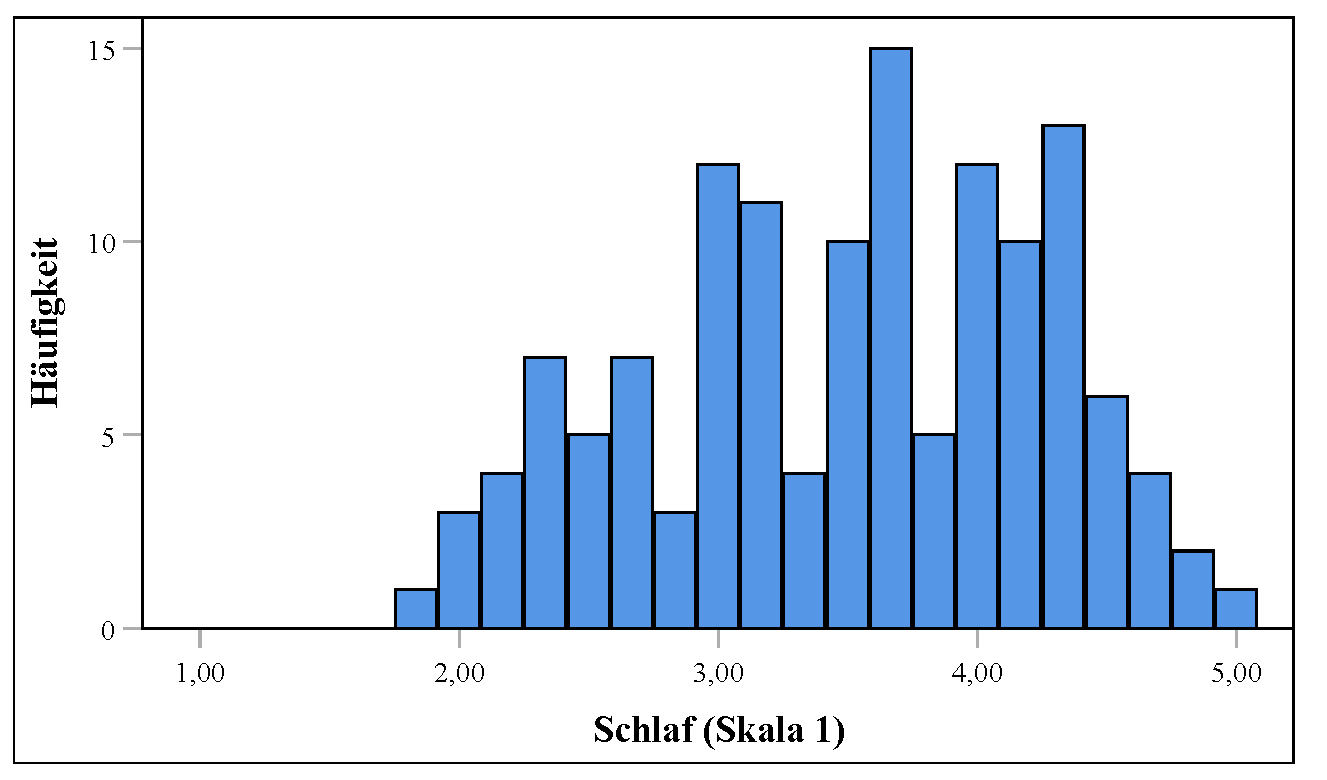
\includegraphics[width=0.8\linewidth]{Histogramm Skala Schlaf.pdf}
        \caption[Histogramm für die Skala Schlaf]{Histogramm für die Skala Schlaf. 
        Codierung: 1.00 = stimme nicht zu ... 5.00~=~stimme vollständig zu. $N = 135$. 
        $M = 3.50$, $SD = 0.76$, $Skewness = -0.25$, $Kurtosis = 0.86$, 
        Cronbachs-\textalpha \ = .72.}
        \label{Histogramm Skala Schlaf}
\end{figure}

Die in dem Histogramm in Abbildung~\ref{Histogramm Skala Ernährung} erkennbare 
Häufigkeitsverteilung ist leicht linksschief (\textit{Skewness} = -0.27) bei einer 
spitzgipfligen Wölbung ($Kurtosis~=~0.65$) und zeigt eine statistisch signifikante 
Abweichung von der Normalverteilung (K-S-Anpassungstest: $p = .008$). Die Mehrheit 
der Befragten berichtet im Durchschnitt somit eher teilweise den Items der 
Ernährungs-Skala zuzustimmen.
\input{Histogramm Skala 2 Ernährung.tex}